\documentclass[a4paper,11pt]{article}
\usepackage{amssymb}
\usepackage{booktabs}
\usepackage{geometry}
\usepackage{color}
\usepackage{hyperref}
\usepackage{listings}
\usepackage{graphicx}
\usepackage{float}
\usepackage{caption}
\usepackage{subcaption}
\usepackage[T1]{fontenc}
\usepackage{algo}

\geometry{
	includeheadfoot,
	margin=2.54cm
}

\setlength\parindent{24pt}

\title{
	2IL76 Algorithms for Geographic Data Set 3 \\
}
\author{
	Bram Kohl - b.j.e.kohl@student.tue.nl - 0746107
}
\date{\today}

\begin{document}
	\maketitle
	
\section*{Exercise 1}
It is neither monotone decreasing, nor increasing. Take for example figure \ref{fig:trajectory1}.

\section*{Exercise 2}
We are given the trajectory and the subcurve for which we have to find recurrences. We can do this by creating a free space diagram, with on the horizontal axis the points in the given trajectory (A[i,j]) and on the vertical axis all other points. Then we fill this diagram by checking for each of the $n-l$ points on the vertical axis whether it is close to any of the $l$ points in the given trajectory ($< \varepsilon$), and coloring the cell in the diagram black if not. We add an extra row for A[i,j] with all black cells, to prevent finding a solution that jumps from A[i-1] to A[j+1] (more on how we find this solution later).\\

Take for example the curve in figure \ref{fig:curve1}, with $i = 2$ and $j = 3$. Now we would expect $a_2$ to be close to $a_6$ and $a_3$ to be close to $a_7$. Of course, this depends on $\varepsilon$, but let's assume $\varepsilon$ is of a size where this is the case, and no other points are close to $a_2$ or $a_3$.

\begin{figure}[H]
	\centering
	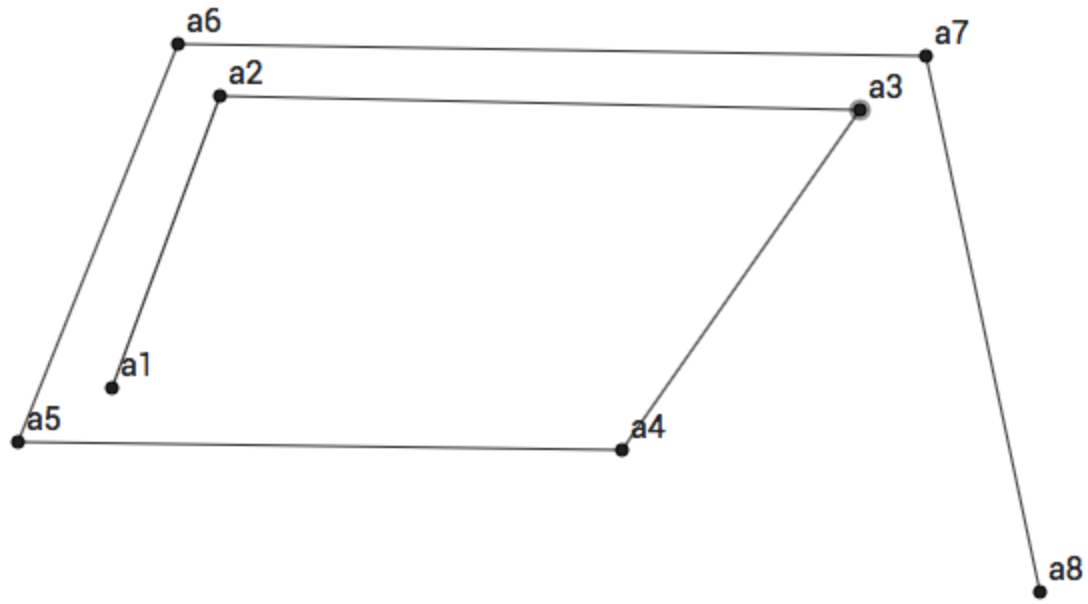
\includegraphics[scale=0.5]{curve1}
	\caption{Curve with recurring subcurve}
	\label{fig:curve1}
\end{figure}

Applying the algorithm that creates the free space diagram then results in the free space diagram of figure \ref{fig:freespace}.

\begin{figure}[H]
	\centering
	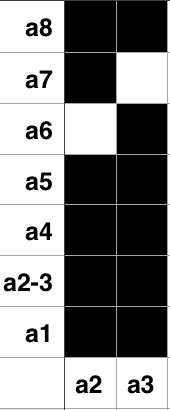
\includegraphics[scale=0.8]{freespace}
	\caption{Free space diagram for figure \ref{fig:curve1}}
	\label{fig:freespace}
\end{figure}

Now, in order to find a solution, we find the lowest free cell in the A[i] column, which in the example is cell ($a_6$,$a_2$). Then we try finding a subcurve by traversing the diagram, prioritizing going to the cell on the right over going to the cell on the top right, and going to the cell one the top right over going to the cell above. We do this to maximize $m$, as we cannot use an A[i] in multiple subcurves, so if we go up, that cell can no longer be used in another subcurve. When we find a subcurve (that is, we get to the $a_j$ column), we start looking for another subcurve with a small enough Fr\'{e}chet distance. We do this by again finding the lowest free cell in the A[i] column, but this time we only look above the cells we used. So in the example we would start looking at $a_7$, which is not free, so we look at $a_8$ which is not free either, so we conclude there are no more subcurves which are close enough to A[i,j]. When we do find such a free cell, we repeat the same process of going right, up right or up.

\subsection*{Proof of correctness}
In order to prove the correctness of our solution, we need to show that the subcurves we find meet the requirements of having a small enough Fr\'{e}chet distance to A[i,j] and being disjoint, as well as show that there is no greater set of subcurves which meet these requirements.\\

For the first part, let's first show that the Fr\'{e}chet distance is small enough. When we find a subcurve A[$i_k$,$j_k$] in the free space diagram, we found it by going to the right, the top right and/or up. So the first vertex of the subcurve, A[$i_k$], is close to A[i]. Then we can separate three cases: we go right, in which case A[$i_k$] is close to A[i+1] as well, we go to the top right, in which case A[$i_k+1$] is close to A[i+1], or we go up, in which case A[$i_k+1$] is close to A[i]. As we stop and add the subcurve only when we reach the A[j] column, and every point in between was close to a point in the other subcurve, the subcurves are close enough to eachother. We do not go back in time in any of the three possible steps (we don't go down or left), so the Fr\'{e}chet distance is small enough.\\
The found subcurves are disjoint, as when we find a subcurve, we continue one row above the last cell in the found subcurve (and this is the highest cell as we never went down). So we can never use one of the used vertices in a new subcurve.\\

What is left to prove is that we find the maximal number of subcurves (maximum $m$) in this way. This is the case, as we go right as much as possible. Only when this is not possible we go upright and when that is not possible either, we go up. So we find the lowest possible subcurve first, and then find the lowest one above that, etc. So using this greedy approach we find the maximum number of subcurves that meet the constraints.

\subsection*{Running time}
Creating the free space diagram just means checking whether the distance between each of the $n-l$ points that are not in the given subcurve A[i,j] and each of the $l$ points in A[i,j] is less than $\varepsilon$. This takes O($nl-l^2$) time. Traversing the free space diagram takes at most O($n-l + l$) = O($n$) time, as we never go down or left.

\end{document} 